\documentclass{article}
\usepackage{amsmath}
\usepackage{graphicx} % Required for inserting images

\title{Homework 3}
\author{Keiver Pabula CHENKEHUI 3210300365}

\begin{document}
\maketitle


\section{Problem 1}
\( p(x) \) is a cubic polynomial, let:
\[
p(x) = a x^3 + b x^2 + c x + d.
\]

Since \( s(0) = 0 \), we have:
\[
p(0) = a(0)^3 + b(0)^2 + c(0) + d = d = 0.
\]
Thus:
\[
p(x) = a x^3 + b x^2 + c x.
\]

To ensure that \( s(x) \) remains continuous and that its first and second derivatives are continuous at \( x = 1 \), we impose the following conditions:
- \( p(1) = (2 - 1)^3 = 1 \),
- \( p'(1) = \frac{d}{dx} (2 - x)^3 \Big|_{x=1} = -3 \),
- \( p''(1) = \frac{d^2}{dx^2} (2 - x)^3 \Big|_{x=1} = 6 \).

This translates into the equations:
\[
a(1)^3 + b(1)^2 + c(1) = a + b + c = 1,
\]
\[
3a(1)^2 + 2b(1) + c = 3a + 2b + c = -3,
\]
\[
6a(1) + 2b = 6a + 2b = 6 \Rightarrow 3a + b = 3.
\]

\[
\begin{cases}
a + b + c = 1, \\
3a + 2b + c = -3, \\
3a + b = 3.
\end{cases}
\]
So we can get
\[
a = 7, \quad b = -18, \quad c = 12.
\]

Thus, we have:
\[
p(x) = 7x^3 - 18x^2 + 12x.
\]
Calculating the second derivative:
\[
p''(x) = 42x - 36.
\]
- \( p''(0) = 42(0) - 36 = -36 \neq 0 \),
- \( p''(2) = 42(2) - 36 = 84 - 36 = 48 \neq 0 \).

Therefore, \( s(x) \) is not a natural cubic spline.


\section{Problem 2}
\subsection{Problem A}
\[
p_i(x) = a_i (x - x_i)^2 + b_i (x - x_i) + c_i,
\]
where there are \( 3(n - 1) \) unknown coefficients \( a_i, b_i, c_i \) for \( n - 1 \) subintervals.

At each interior point \( x_i \), the spline must be continuous:
   \[
   p_i(x_i) = p_{i+1}(x_i) \quad \text{for all } i = 2, 3, \dots, n - 1.
   \]
   This provides \( n - 2 \) equations.

At each interior point \( x_i \), the first derivative of the spline must also be continuous:
   \[
   p_i'(x_i) = p_{i+1}'(x_i) \quad \text{for all } i = 2, 3, \dots, n - 1.
   \]
   This provides another \( n - 2 \) equations.

- Total number of unknowns: \( 3(n - 1) \).
- Total number of equations: \( 2(n - 2) \).

Since there are fewer equations than unknowns, an additional condition is required.

\subsection{Problem B}
\[
p_i(x) = a_i (x - x_i)^2 + b_i (x - x_i) + c_i.
\]
Given:
\[
p_i(x_i) = f_i, \quad p_i(x_{i+1}) = f_{i+1}, \quad p_i'(x_i) = m_i.
\]

From \( p_i(x_i) = a_i (x_i - x_i)^2 + b_i (x_i - x_i) + c_i = c_i = f_i \), we get:
\[
c_i = f_i.
\]
The first derivative:
\[
p_i'(x) = 2a_i (x - x_i) + b_i.
\]
At \( x_{i+1} \):
\[
p_i'(x_{i+1}) = 2a_i (x_{i+1} - x_i) + b_i = m_i.
\]
Using:
\[
a_i (x_{i+1} - x_i)^2 + m_i (x_{i+1} - x_i) + f_i = f_{i+1},
\]
we find:
\[
a_i = \frac{f_{i+1} - f_i - m_i (x_{i+1} - x_i)}{(x_{i+1} - x_i)^2}.
\]

Thus:
\[
p_i(x) = \frac{f_{i+1} - f_i - m_i (x_{i+1} - x_i)}{(x_{i+1} - x_i)^2} (x - x_i)^2 + m_i (x - x_i) + f_i.
\]

\subsection{Problem C}
Since:
\[
p_i'(x_{i+1}) = p_{i+1}'(x_{i+1}),
\]
we have a system of equations involving \( m_2, m_3, \ldots, m_{n-1} \). Combining these equations with the known initial derivative \( m_1 \), we can solve for all \( m_i \). This allows us to uniquely determine the quadratic spline \( s \).



\section{Problem 3}
Given:
\[
s_1(x) = 1 + c (x + 1)^3,
\]
\[
s_1'(x) = 3c (x + 1)^2,
\]
\[
s_1''(x) = 6c (x + 1).
\]

To satisfy \( s_1''(-1) = 0 \):
\[
s_1''(-1) = 6c (-1 + 1) = 0 \implies c = 0.
\]

Let \( s_2(x) \) be a cubic polynomial:
\[
s_2(x) = a x^3 + b x^2 + d x + e.
\]

\( s_1(0) = s_2(0) \):
   \[
   s_1(0) = 1 + c (0 + 1)^3 = 1 + c \implies e = 1 + c = s_2(0).
   \]

\( s_1'(0) = s_2'(0) \):
   \[
   s_2'(x) = 3a x^2 + 2b x + d,
   \]
   \[
   s_1'(0) = 3c (0 + 1)^2 = 3c \implies d = 3c = s_2'(0).
   \]
\( s_1''(0) = s_2''(0) \):
   \[
   s_2''(x) = 6a x + 2b,
   \]
   \[
   s_1''(0) = 6c (0 + 1) = 6c \implies 2b = 6c \implies b = 3c.
   \]

\[
s_2''(1) = 6a (1) + 2b = 6a + 2(3c) = 6a + 6c = 0 \implies a = -c.
\]

Using the condition \( s_2(1) = -1 \):
\[
s_2(1) = a(1)^3 + b(1)^2 + d(1) + e = -c + 3c + 3c + (1 + c) = 6c + 1,
\]
\[
6c = -2 \implies c = -\frac{1}{3}.
\]

The constant \( c = -\frac{1}{3} \), and:
\[
s_2(x) = -\frac{1}{3} x^3 + x^2 - x + \frac{2}{3}.
\]


\section{Problem 4}
\subsection{Problem a}
We aim to find the natural cubic spline interpolation for the function \( f(x) = \cos\left(\frac{\pi}{2} x\right) \) on the interval \([-1, 1]\):
\begin{itemize}
    \item \( f(-1) = \cos\left(-\frac{\pi}{2}\right) = 0 \),
    \item \( f(0) = \cos(0) = 1 \),
    \item \( f(1) = \cos\left(\frac{\pi}{2}\right) = 0 \).
\end{itemize}

Define \( s_1(x) \) on \([-1, 0]\) as:
\[
s_1(x) = a_1 x^3 + b_1 x^2 + c_1 x + d_1.
\]
Define \( s_2(x) \) on \([0, 1]\) as:
\[
s_2(x) = a_2 x^3 + b_2 x^2 + c_2 x + d_2.
\]

\( s_1''(-1) = 0 \):
   \[
   s_1''(x) = 6a_1 x + 2b_1 \implies s_1''(-1) = 6a_1(-1) + 2b_1 = -6a_1 + 2b_1 = 0 \implies b_1 = 3a_1.
   \]
\( s_2''(1) = 0 \):
   \[
   s_2''(x) = 6a_2 x + 2b_2 \implies s_2''(1) = 6a_2(1) + 2b_2 = 6a_2 + 2b_2 = 0 \implies b_2 = -3a_2.
   \]

\( s_1(0) = s_2(0) = 1 \):
   \[
   s_1(0) = a_1 \cdot 0^3 + b_1 \cdot 0^2 + c_1 \cdot 0 + d_1 = d_1 = 1,
   \]
   \[
   s_2(0) = a_2 \cdot 0^3 + b_2 \cdot 0^2 + c_2 \cdot 0 + d_2 = d_2 = 1.
   \]

\( s_1'(0) = s_2'(0) \):
   \[
   s_1'(x) = 3a_1 x^2 + 2b_1 x + c_1 \implies s_1'(0) = 3a_1 \cdot 0^2 + 2b_1 \cdot 0 + c_1 = c_1,
   \]
   \[
   s_2'(x) = 3a_2 x^2 + 2b_2 x + c_2 \implies s_2'(0) = 3a_2 \cdot 0^2 + 2b_2 \cdot 0 + c_2 = c_2.
   \]
   Therefore, \( c_1 = c_2 \).

\( s_1''(0) = s_2''(0) \):
   \[
   s_1''(0) = 2b_1, \quad s_2''(0) = 2b_2 \implies b_1 = b_2.
   \]

Using these conditions, we obtain:
\[
s_1(x) = -\frac{1}{2} x^3 + \frac{3}{2} x^2 + 1,
\]
\[
s_2(x) = \frac{1}{2} x^3 - \frac{3}{2} x^2 + 1.
\]

\subsection{Problem b}
1. \( g(-1) = 0 \):
   \[
   a(-1)^2 + b(-1) + c = 0 \implies a - b + c = 0.
   \]
2. \( g(0) = 1 \):
   \[
   a(0)^2 + b(0) + c = 1 \implies c = 1.
   \]
3. \( g(1) = 0 \):
   \[
   a(1)^2 + b(1) + c = 0 \implies a + b + c = 0.
   \]

Substituting \( c = 1 \) into the first and third equations:
\[
a - b + 1 = 0 \implies a - b = -1,
\]
\[
a + b + 1 = 0 \implies a + b = -1.
\]

Solving this system:
\[
2a = -2 \implies a = -1,
\]
\[
2b = 0 \implies b = 0.
\]

Thus:
\[
g(x) = -x^2 + 1.
\]

\[
\int_{-1}^1 \left( g''(x) \right)^2 \, dx = \frac{8}{3}.
\]

Calculate \( s''(x) \) and the bending energy:
\[
\int_{-1}^1 \left( s''(x) \right)^2 \, dx = \int_{-1}^0 \left( -3x - 3 \right)^2 \, dx + \int_{0}^1 \left( 3x - 3 \right)^2 \, dx > 6.
\]

Verifying that the bending energy of the natural cubic spline is smaller, confirming that natural cubic splines minimize the total bending energy.


\section{Problem 5}
\subsection{Problem A}

The first-degree B-spline \( B_i^1(x) \) is defined as:
\[
B_i^1(x) = \begin{cases}
\frac{x - t_{i-1}}{t_i - t_{i-1}} & \text{if } x \in [t_{i-1}, t_i], \\[10pt]
\frac{t_{i+1} - x}{t_{i+1} - t_i} & \text{if } x \in [t_i, t_{i+1}], \\[10pt]
0 & \text{otherwise}.
\end{cases}
\]

The next B-spline \( B_{i+1}^1(x) \) is given by:
\[
B_{i+1}^1(x) = \begin{cases}
\frac{x - t_i}{t_{i+1} - t_i} & \text{if } x \in [t_i, t_{i+1}], \\[10pt]
\frac{t_{i+2} - x}{t_{i+2} - t_{i+1}} & \text{if } x \in [t_{i+1}, t_{i+2}], \\[10pt]
0 & \text{otherwise}.
\end{cases}
\]

Using the recursive formula, the second-degree B-spline \( B_i^2(x) \) is:
\[
B_i^2(x) = \frac{x - t_i}{t_{i+2} - t_i} B_i^1(x) + \frac{t_{i+2} - x}{t_{i+2} - t_{i+1}} B_{i+1}^1(x),
\]
which gives:
\[
B_i^2(x) = \begin{cases} 
\frac{(x - t_{i-1})^2}{(t_{i+1} - t_{i-1})(t_i - t_{i-1})} & \text{if } x \in [t_{i-1}, t_i], \\[10pt]
\frac{(t_{i+2} - x)(x - t_i)}{(t_{i+2} - t_i)(t_{i+1} - t_i)} & \text{if } x \in [t_i, t_{i+1}], \\[10pt]
\frac{(t_{i+2} - x)^2}{(t_{i+2} - t_i)(t_{i+2} - t_{i+1})} & \text{if } x \in [t_{i+1}, t_{i+2}], \\[10pt]
0 & \text{otherwise}.
\end{cases}
\]

\subsection{Problem B}

We compute \( \frac{d}{dx} B_i^2(x) \) piecewise for the intervals \( [t_{i-1}, t_i], [t_i, t_{i+1}], [t_{i+1}, t_{i+2}] \):

1. At \( x = t_i \):
   \[
   p_1(t_i) = \frac{2(t_i - t_{i-1})}{(t_{i+1} - t_{i-1})(t_i - t_{i-1})} = \frac{2}{t_{i+1} - t_{i-1}} = p_2(t_i).
   \]

2. At \( x = t_{i+1} \), ensure \( p_2(t_{i+1}) = p_3(t_{i+1}) \):
   \[
   p_3(t_{i+1}) = \frac{2(t_{i+2} - t_{i+1})}{(t_{i+2} - t_i)(t_{i+2} - t_{i+1})} = \frac{-2}{t_{i+2} - t_i} = p_2(t_{i+1}).
   \]

Hence, \( \frac{d}{dx} B_i^2(x) \) is continuous at \( x = t_i \) and \( x = t_{i+1} \).

\subsection{Problem C}

The derivative \( \frac{d}{dx} B_i^2(x) \) is positive on \( (t_{i-1}, t_i) \) and negative on \( (t_i, t_{i+1}) \), indicating a unique extremum point \( x^* \) within \( (t_i, t_{i+1}) \).

We solve for \( x^* \) such that:
\[
\frac{t_{i+1} + t_{i-1} - 2x^*}{t_{i+1} - t_{i-1}} + \frac{t_{i+2} + t_i - 2x^*}{t_{i+2} - t_i} = 0.
\]
Solving for \( x^* \):
\[
x^* = \frac{t_i t_{i+2} + t_i t_{i+1} - t_{i-1} t_i}{(t_{i+2} + t_{i+1}) - (t_i + t_{i-1})}.
\]

\subsection{Problem D}

The function \( B_i^2(x) \) is zero at \( t_{i-1} \) and \( t_{i+2} \), and it achieves a maximum value between these points. The peak value at \( x^* \) is less than 1, ensuring \( B_i^2(x) \in [0, 1] \).

\subsection{Problem E}
\begin{figure}[h] % 'h' 表示将图片放在当前段落
    \centering
    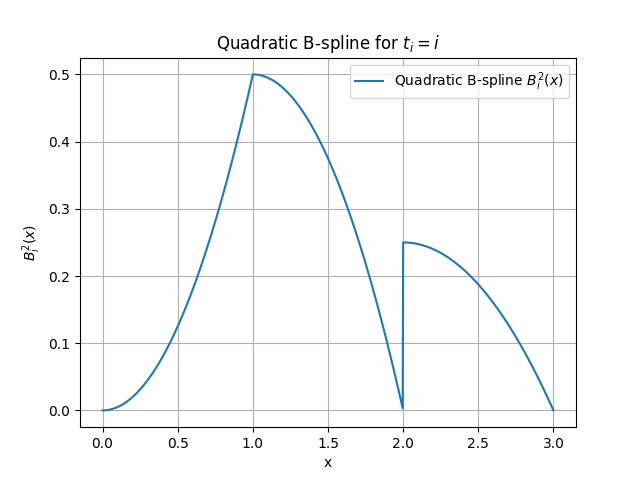
\includegraphics[width=0.5\textwidth]{Figure_1.png} 
    \label{fig:sample_image} % 添加标签以便在文中引用
\end{figure}




\section{Problem 6}
Given:
\[
[t_{i-1}, t_i, t_{i+1}, t_{i+2}]f = \frac{[t_i, t_{i+1}, t_{i+2}]f - [t_{i-1}, t_i, t_{i+1}]f}{t_{i+2} - t_{i-1}},
\]
for \( f(x) = (t - x)^2_+ \).

We have:
\[
B_i^2(x) = \frac{x - t_{i-1}}{t_{i+1} - t_{i-1}} B_i^1(x) + \frac{t_{i+2} - x}{t_{i+2} - t_i} B_{i+1}^1(x),
\]
where \( B_i^1(x) \) and \( B_{i+1}^1(x) \) are the first-degree B-splines. The explicit expression for a first-degree B-spline is:

\[
B_i^1(x) = \begin{cases} 
\frac{x - t_{i-1}}{t_i - t_{i-1}}, & \text{if } t_{i-1} \leq x < t_i, \\[10pt]
\frac{t_{i+1} - x}{t_{i+1} - t_i}, & \text{if } t_i \leq x < t_{i+1}, \\[10pt]
0, & \text{otherwise}.
\end{cases}
\]

Using the recursive definition, we have:
\begin{align*}
B_i^2(x) &= (x - t_{i-1})[t_{i-1}, t_i, t_{i+1}] (t - x)_+^1 + (t_{i+2} - x)[t_i, t_{i+1}, t_{i+2}] (t - x)_+^1 \\
&= -[t_{i-1}, t_i, t_{i+1}] (t - x)_+^2 + [t_i, t_{i+1}, t_{i+2}] (t - x)_+^2 \\
&= (t_{i+2} - t_{i-1}) [t_{i-1}, t_i, t_{i+1}, t_{i+2}] (t - x)_+^2.
\end{align*}

Thus, we obtain:
\[
(t_{i+2} - t_{i-1})[t_{i-1}, t_i, t_{i+1}, t_{i+2}] (t - x)^2_+ = B_i^2(x).
\]
Q.E.D.



\section{Problem 7}
Given:
\[
\frac{d}{dx} B_i^{n+1}(x) = (n+1) \left( \frac{B_i^n(x)}{t_{i+n} - t_{i-1}} - \frac{B_{i+1}^n(x)}{t_{i+n+1} - t_i} \right), \quad n \geq 1.
\]

Integrate both sides over the support interval \( [t_{i-1}, t_{i+n+1}] \):
\[
\int_{t_{i-1}}^{t_{i+n+1}} \frac{d}{dx} B_i^{n+1}(x) \, dx = \int_{t_{i-1}}^{t_{i+n+1}} \left( \frac{(n+1) B_i^n(x)}{t_{i+n} - t_{i-1}} - \frac{(n+1) B_{i+1}^n(x)}{t_{i+n+1} - t_i} \right) \, dx.
\]

This simplifies to:
\[
B_i^{n+1}(t_{i+n+1}) - B_i^{n+1}(t_{i-1}) = (n+1) \left( \int_{t_{i-1}}^{t_{i+n}} \frac{B_i^n(x)}{t_{i+n} - t_{i-1}} \, dx - \int_{t_i}^{t_{i+n+1}} \frac{B_{i+1}^n(x)}{t_{i+n+1} - t_i} \, dx \right).
\]

Simplifying further:
\[
0 = \int_{t_i}^{t_{i+n+1}} \frac{B_{i+1}^n(x)}{t_{i+n+1} - t_i} \, dx.
\]

Hence, we conclude that the scaled integral of the B-spline \( B_i^n(x) \) over its support interval is independent of the index \( i \).


\section{Problem 8}
\subsection{Problem A}
Let:
\[
e_2(x_1, x_2, x_3, x_4) = x_1x_2 + x_1x_3 + x_1x_4 + x_2x_3 + x_2x_4 + x_3x_4.
\]

The divided difference is defined as:
\[
[x_i, x_j]f = \frac{f(x_i) - f(x_j)}{x_i - x_j}.
\]

Here, \( f(x) = x \), and we express the following using binomial terms:
\begin{itemize}
    \item \( [x_1, x_2] \): Represents the product \( x_1 x_2 \),
    \item \( [x_1, x_3] \): Represents the product \( x_1 x_3 \),
    \item \( [x_1, x_4] \): Represents the product \( x_1 x_4 \),
    \item \( [x_2, x_3] \): Represents the product \( x_2 x_3 \),
    \item \( [x_2, x_4] \): Represents the product \( x_2 x_4 \),
    \item \( [x_3, x_4] \): Represents the product \( x_3 x_4 \).
\end{itemize}

Thus:
\[
e_2(x_1, x_2, x_3, x_4) = x_1x_2 + x_1x_3 + x_1x_4 + x_2x_3 + x_2x_4 + x_3x_4.
\]

By computing the above divided differences and adding these terms, we observe that all pairwise products appear in the complete symmetric polynomial. Hence, the theorem holds for \( m = 4 \) and \( n = 2 \).

\section{ Problem B}
\[
(x_{i+n+1} - x_i) \sigma_{m-n-1}(x_i, \dots, x_{i+n+1})
\]
\[
= \sigma_{m-n}(x_i, \dots, x_{i+n+1}) - \sigma_{m-n}(x_i, \dots, x_{i+n}) - x_i \sigma_{m-n-1}(x_i, \dots, x_{i+n+1}).
\]
This simplifies to:
\[
= \sigma_{m-n}(x_{i+1}, \dots, x_{i+n+1}) - \sigma_{m-n}(x_i, \dots, x_{i+n}).
\]

For \( n = 0 \):
\[
\sigma_m(x_i) = [x_i] x_i^m = x_i^m.
\]

Assume it holds for \( k = n \), and consider the case for \( k = n + 1 \):
\[
\sigma_{m-n-1}(x_i, \dots, x_{i+n+1}) = \frac{\sigma_{m-n}(x_i, \dots, x_{i+n+1}) - \sigma_{m-n}(x_i, \dots, x_{i+n})}{x_{i+n+1} - x_i}.
\]
This can be rewritten as:
\[
= \frac{[x_{i+1}, \dots, x_{i+n+1}] x^m - [x_i, \dots, x_{i+n}] x^m}{x_{i+n+1} - x_i} = [x_i, x_{i+1}, \dots, x_{i+n+1}] x^m.
\]

Thus, the proof is complete.

\end{document}
